\section{Mes premiers pas}
\subsection*{Présentation du perceptron}
C'est  en 1943, que McCulloch et Pitts introduisent le modèle du perceptron. Ce modèle est basé sur le fonctionnement du neurone humain.

\begin{figure}[htbp!]
    \begin{subfigure}[]{0.5\textwidth}
        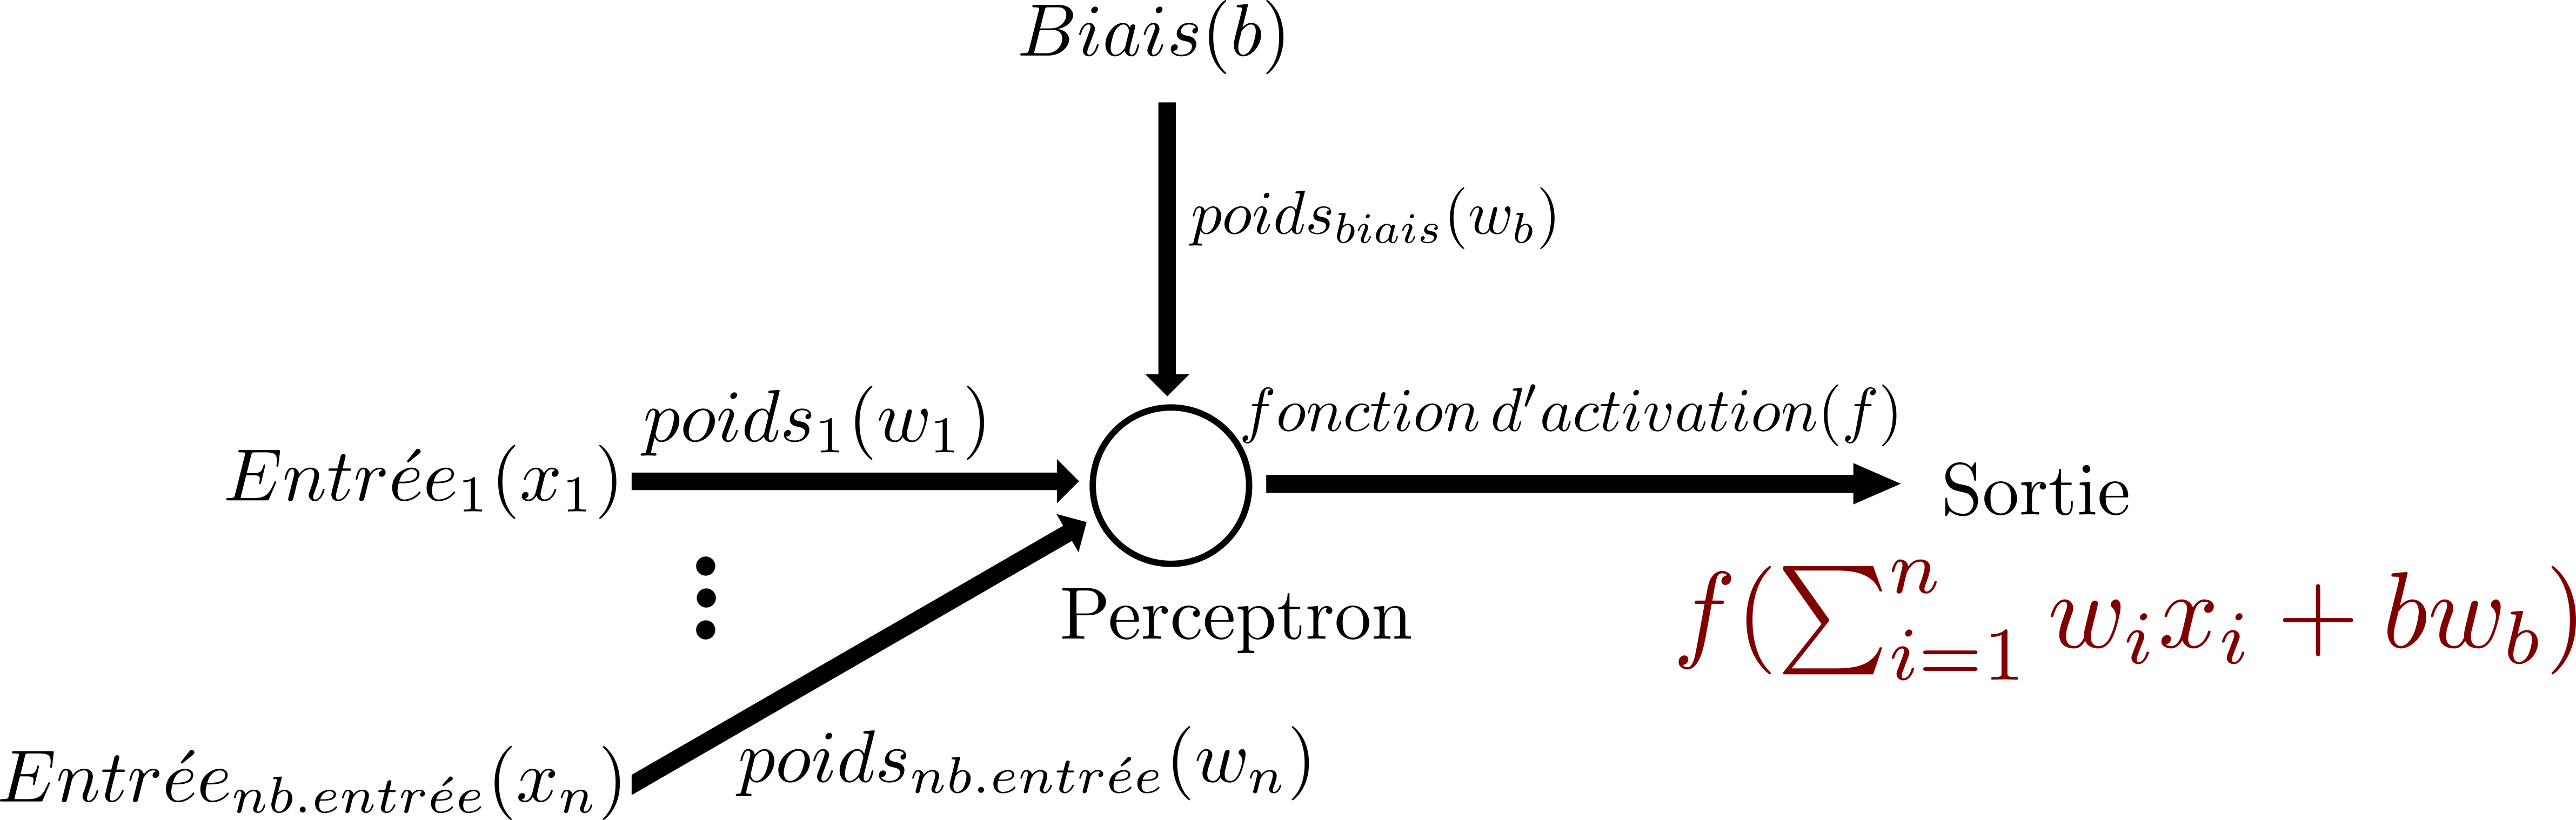
\includegraphics[width=\textwidth]{1-Perceptron.png}
        \caption{Schéma d'un perceptron}
    \end{subfigure}
    \begin{subfigure}[]{0.5\textwidth}
        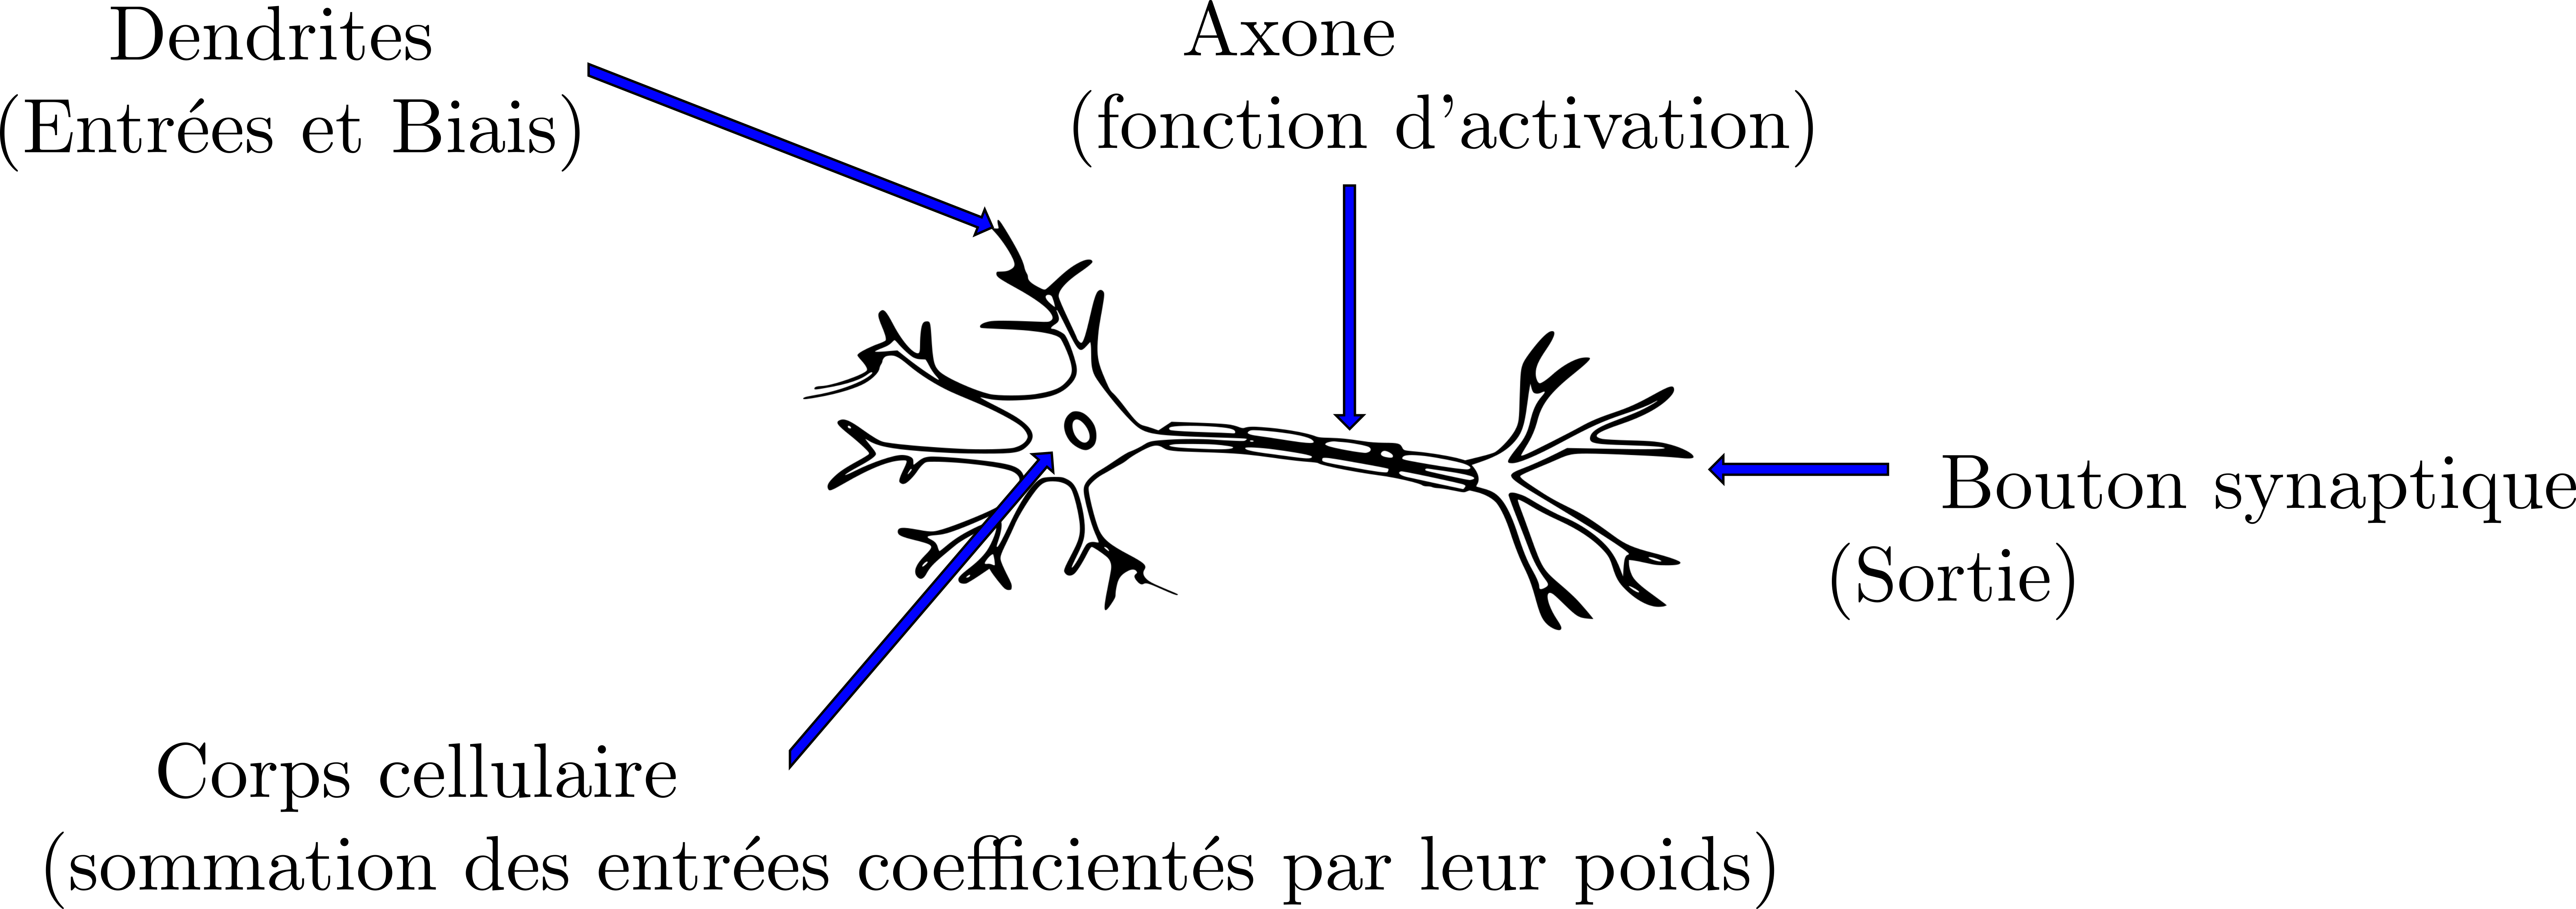
\includegraphics[width=\textwidth]{2-Neurone.png}
        \caption{Schéma d'un neurone humain}
    \end{subfigure}
\end{figure}

Nous représenterons informatiquement une couche de perceptron sous forme de matrice. \newline
\begin{center}
    \centering
    $
        f
        \left(
        \begin{pmatrix}
            x_1 & \ldots & x_n & b
        \end{pmatrix}
        \times
        \begin{pmatrix}
            w_1    \\
            \vdots \\
            w_n    \\
            w_b
        \end{pmatrix}
        \right)
    $ \\
\end{center}